\section{On-FPGA Checker}
\label{sec:on-fpga-checker}

We next map the trained bitstream classifier into FPGA logic and consider how
the resulting checker can be placed in the Coyote deployment path. The hardware
design consists of two components: deterministic byte-stream preprocessing and
the quantized CNN classifier. Importantly, both execute on the FPGA, allowing inspection to
take place without a separate host-side classification stage.

\subsection{Hardware Generation}
\label{sec:hardware-generation}

We convert the trained QKeras CNN to hardware using
hls4ml~\cite{duarte2018fast,aarrestad2021fast}. hls4ml translates the quantized
network into an HLS implementation, which is first evaluated through C
simulation and subsequently synthesized to RTL. The final models use
quantization-aware training, so the weight and activation precision used during
training already reflects the W8A8 representation targeted by the generated
hardware.

Before synthesis, we compare the hls4ml C-simulation output against the
corresponding QKeras model. We require matching classifications on the
validation inputs and inspect output deviations before synthesis. This provides
a parity check between the trained model and its fixed-point hardware
implementation.

The preprocessing operation from Section~\ref{sec:method-preprocessing} is
implemented separately in HLS C++ and lowered to RTL. It operates directly on
the incoming bitstream bytes and reproduces the deterministic sampling,
padding, inversion, and normalization used during training. The latency reported
in Section~\ref{sec:eval-hardware} therefore includes both FPGA-side
preprocessing and CNN inference.

\subsection{Hardware Optimization}
\label{sec:hardware-optimization}

Once the trained network is fixed, hls4ml exposes a hardware design space that
trades resource usage against inference latency. The main parameter is the
\emph{reuse factor}, which controls how aggressively arithmetic units are shared
across operations. Lower reuse increases parallelism and reduces latency at the
cost of additional hardware, while higher reuse reduces resource use but
increases execution time.

We initially evaluate resource-oriented hls4ml configurations and sweep reuse
factors for the selected CNN architectures. A single global reuse setting,
however, provides only a coarse tradeoff because convolutional stages differ
substantially in their operation counts and hardware cost. We therefore also
apply manual per-layer reuse settings, assigning greater parallelism to
latency-dominant layers while retaining more sharing elsewhere.

Quantization and pruning are additionally explored as hardware-aware model
transformations. The final checker uses W8A8 quantization trained through
QKeras quantization-aware training. For each transformed model, we retain a
configuration only when software detection quality and hls4ml prediction parity
remain acceptable. Section~\ref{sec:eval-hardware} evaluates the resulting
implementations jointly in terms of detection quality, latency, and routed FPGA
resources.

\subsection{Proposed Coyote Integration}
\label{sec:coyote-integration}

Coyote separates trusted platform services from partially reconfigurable user
regions, providing a natural location for bitstream inspection before
PR~\cite{ramhorst2025coyote}. We propose placing the on-FPGA checker in this
trusted deployment path, as illustrated in
Figure~\ref{fig:coyote-integration}.

An incoming user partial bitstream is first processed by the FPGA-side
preprocessing logic and passed to the synthesized CNN. The CNN produces a
maliciousness score, which trusted deployment logic compares against a configured
threshold. Bitstreams classified as suspicious are rejected, while accepted
bitstreams are allowed to proceed to the Coyote partial-reconfiguration
controller.

\begin{figure*}[t]
\centering
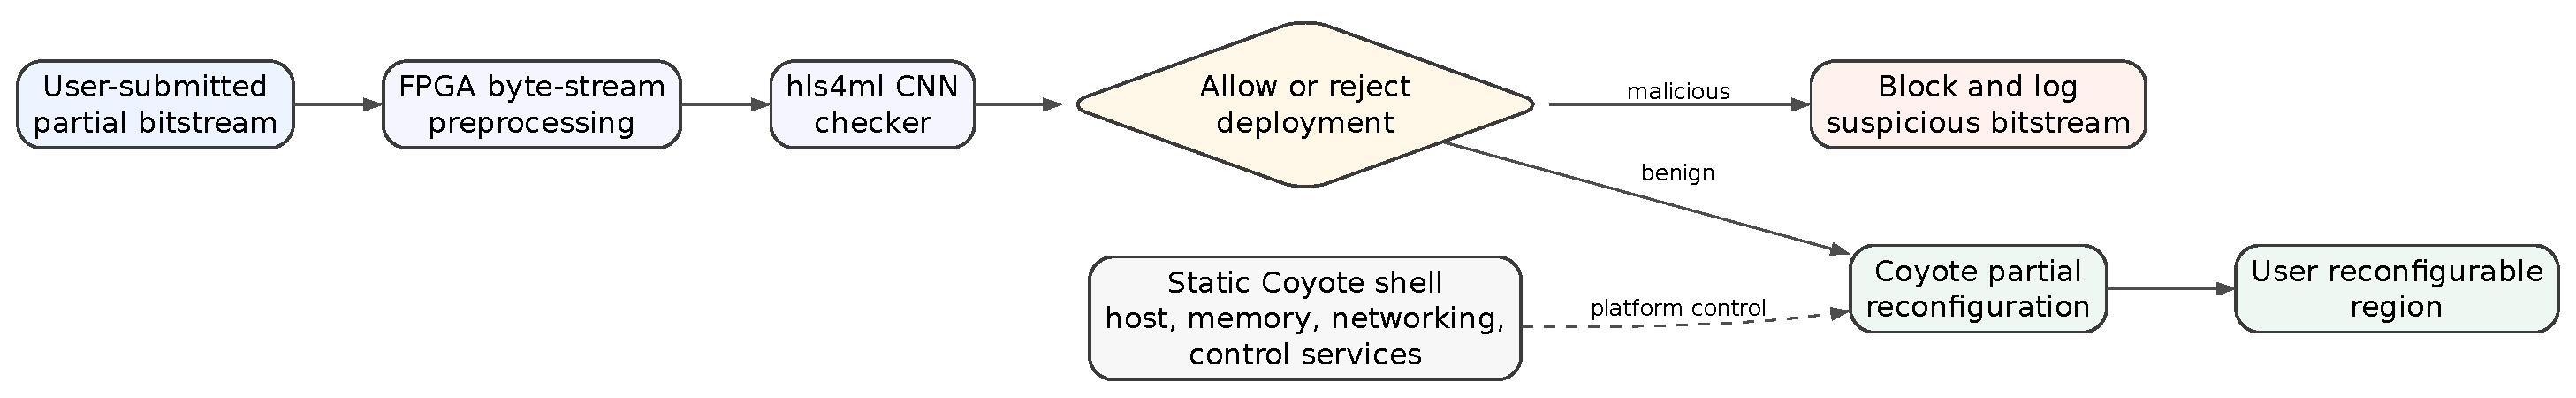
\includegraphics[width=0.95\textwidth]{figures/coyote_integration_path.pdf}
\caption{Proposed integration of the on-FPGA checker into the Coyote
deployment path. FPGA-side preprocessing and CNN inference inspect an
incoming partial bitstream before it is passed to the partial-reconfiguration
controller.}
\label{fig:coyote-integration}
\end{figure*}


The integration shown in Figure~\ref{fig:coyote-integration} is a proposed
deployment architecture rather than a completed end-to-end Coyote
implementation. This work implements and evaluates the FPGA preprocessing and
CNN checker components; connection to Coyote's PR controller and the associated
control-plane logic remain future work.